\newpage
\section{System Model}
\subsection{Backlog}
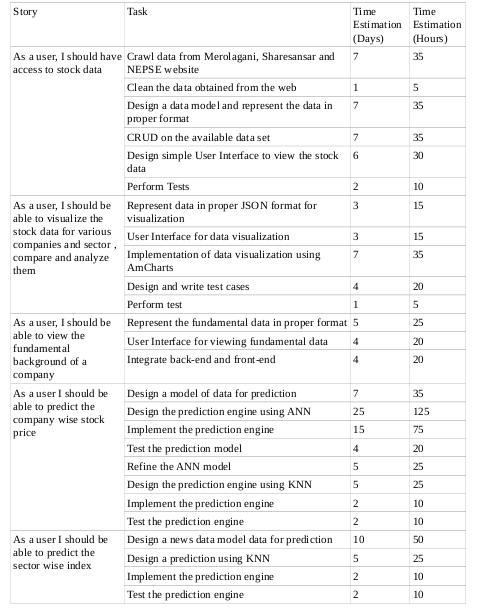
\includegraphics{fig/backlog.png}\\[0.2cm]
%\begin{figure}[h!]
%  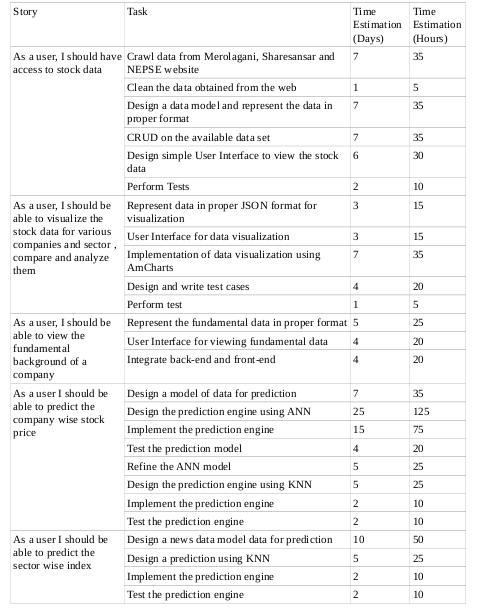
\includegraphics[width=6in]{fig/backlog}
 % \caption{Backlog}\label{fig:Backlog}
%\end{figure}
\subsection{Dataflow Diagram}
The level 0 dataflow diagram is shown in Figure \ref{fig:dfd0}.
\begin{figure}[h!]
  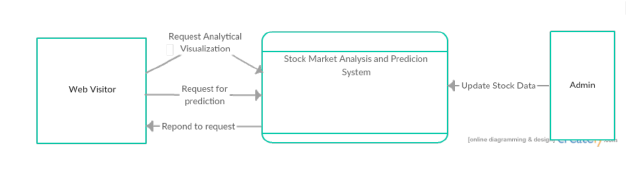
\includegraphics[width=6in]{fig/dfd0}
  \caption{Dfd level 0 }\label{fig:dfd0}
\end{figure}

The level 1 dataflow diagram is shown in Figure \ref{fig:dfd1}.

\begin{figure}[h!]
  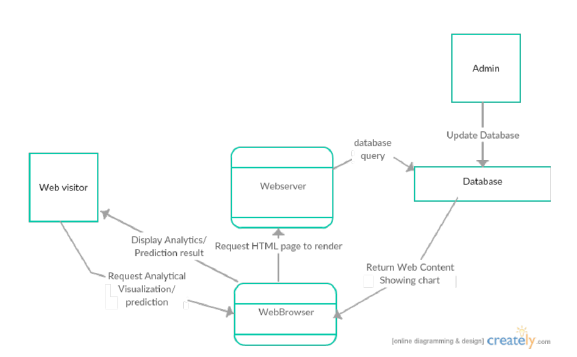
\includegraphics[width=6in]{fig/dfd1}
  \caption{Dfd level 1 }\label{fig:dfd1}
\end{figure}

\newpage
\subsection{Sequence Diagram}
The sequence diagram for the stock prediction is shown below in Figure \ref{fig:sequence}.

\begin{figure}[h!]
  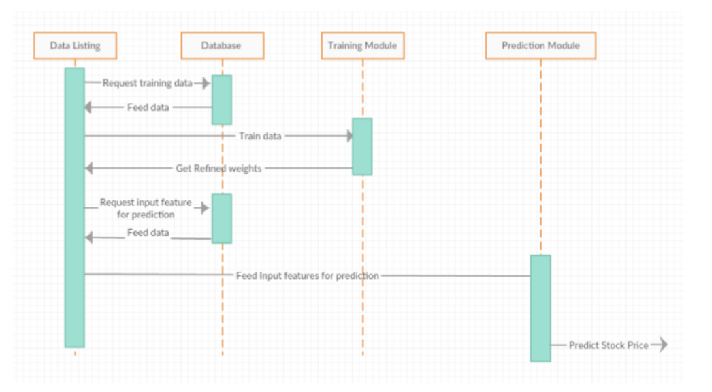
\includegraphics[width=\textwidth]{fig/sequence}
  \caption{Sequence diagram for stock prediction }\label{fig:sequence}
\end{figure}


The sequence diagram for the stock analysis is shown in Figure \ref{fig:sequencevis}.

\begin{figure}[h!]
  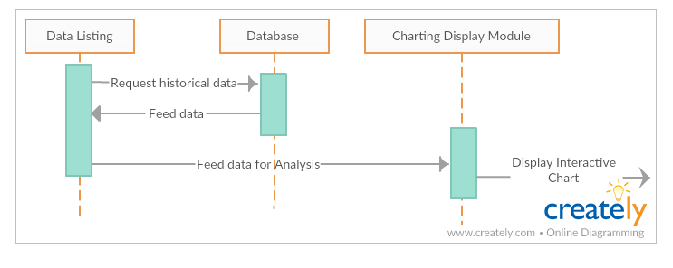
\includegraphics[width=\textwidth]{fig/sequencevis}
  \caption{Sequence diagram for stock analysis }\label{fig:sequencevis}
\end{figure}

\newpage
\subsection{Use Case Modeling}
A use case diagram shows the various actors that can act upon the system and what actions they can perform.
The use case diagram for the system is depicted below in Figure \ref{fig:usecase}.
\begin{figure}[h!]
  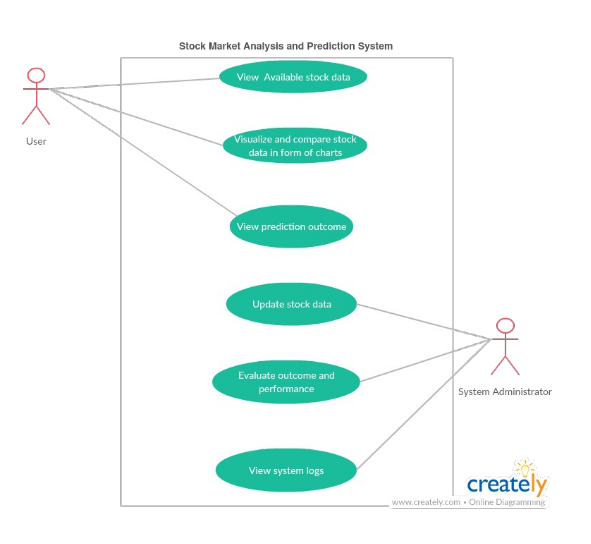
\includegraphics[width=6in]{fig/usecase}
  \caption{Top level usecase diagram for stock market analysis and prediction }\label{fig:usecase}
\end{figure}

\newpage
\subsection{Activity Diagram}
The activity diagram for the system is shown in Figure \ref{fig:activity}.

\begin{figure}[h!]
  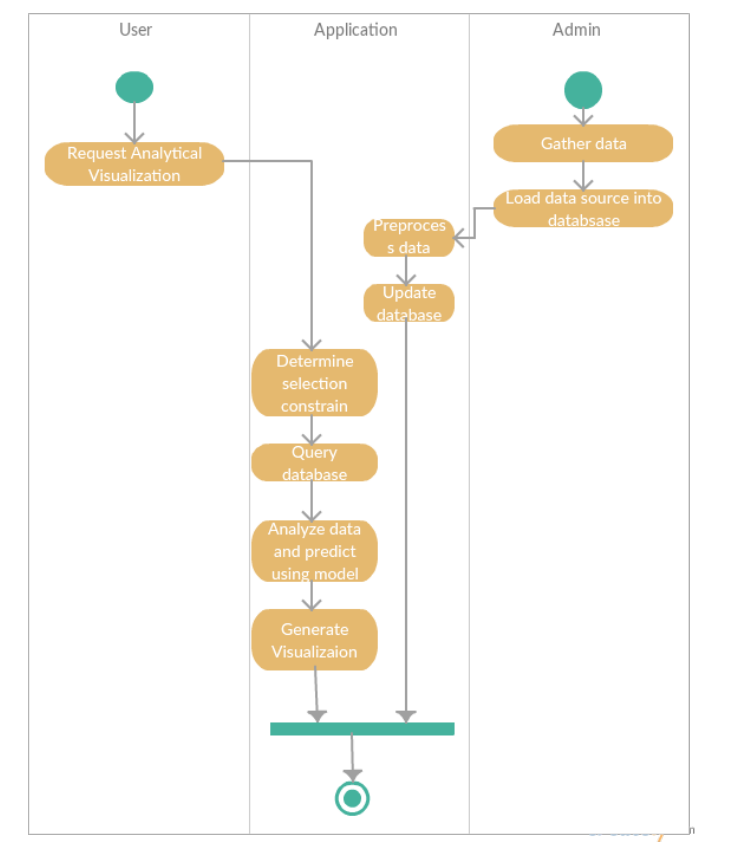
\includegraphics[width=6in]{fig/activity}
  \caption{Activity diagram for stock market analysis and prediction }\label{fig:activity}
\end{figure}

